%% \index{Add!Test Cases}
%% \index{Test Case!Add}
%% For specific information on adding \gdcases{} from the library, see the previous section \bxpref{usingtemplate}. 
%% \begin{enumerate}
%% \item Open the \gdtestcaseeditor{} by double-clicking on the \gdcase{} you want to edit in the \gdtestcasebrowser{}. 
%% \item Select a \gdcase{} via the context-sensitive menu in the \gdtestcasebrowser{} by selecting:
%% \bxmenu{Reference Existing \gdcase{}}{}{}\\

%% \bxtipp{You can also add \gdcases{} by dragging them from the \gdtestcasebrowser{} or by pressing \bxkey{ENTER} on a selected \gdcase{} in the \gdtestcaseeditor{}. You can filter in the \gdtestcasebrowser{} using the field at the top. Use star \bxshell{*} as a wild card.}

%% \item Choose a \gdcase{} or \gdcases{} to add from the dialog which appears (\bxfigref{referencetestcasedialog}).

%% \bxtipp{You can filter in this dialog using the field at the top. Use star \bxshell{*} as a wild card.}

%% \begin{figure}[h]
%% \begin{center}
%% 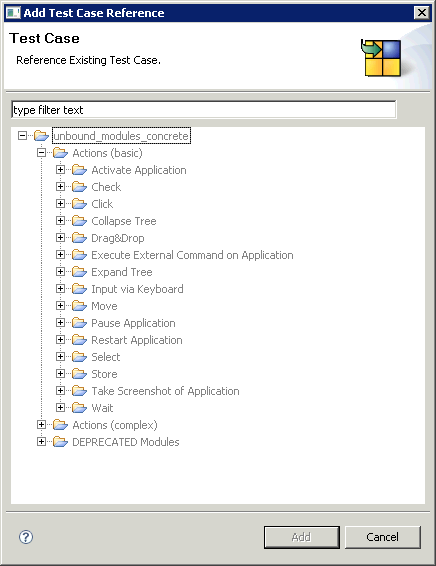
\includegraphics{Tasks/Testcases/PS/referencetestcasedialog}
%% \caption{Add \gdcase{} reference dialog}
%% \label{referencetestcasedialog}
%% \end{center}
%% \end{figure} 

%% \item Click \bxcaption{OK}. 

%% \item The \gdcase{} or \gdcases{} you selected appear(s) in the \gdtestcaseeditor{}. They are marked with a small arrow to show that they are reused (referenced) here. The name of the \gdcase{} is contained in angled brackets (\bxshell{< >}) to show that it is the same name that you used when you specified the \gdcase{}. 
%% \item Save the changes in the editor.
%% \end{enumerate}

%% \bxwarn{You can't add a \gdcase{} which would cause an infinite loop.}
